% **** Szablon pracy magisterskiej, licencjackiej lub inżynierskiej ****

\documentclass[polish,12pt,twoside,a4paper]{report}

% *************** Definicje stylu dokumentu ***************

% *********************************************************************************
% W pliku tym zdefiniowany jest wygl¹d dokumentu.
% Zmiany tutaj nie s¹ konieczne o ile nie zamierzasz zmieniaæ wygl¹du dokumentu.
% *********************************************************************************

% *************** Za³adowanie pakietów ***************
\usepackage[a4paper,twoside,left=2.0cm,right=1.5cm,top=1.5cm,bottom=1.5cm]{geometry}
\usepackage[T1]{fontenc}
%\usepackage[cp1250]{inputenc}
\usepackage[utf8]{inputenc}
\usepackage[polish]{babel}
\usepackage{amsmath}
\usepackage{amsfonts}
\usepackage{graphicx}
\usepackage{graphics}
\usepackage{times}
\usepackage{indentfirst}%wciecia a nowych akapitach
\usepackage{listings}
\usepackage{url}
\usepackage[colorlinks=true, linkcolor=black, urlcolor=black, citecolor=black]{hyperref}

\selectlanguage{polish}

%szerokoœœ wciêæ
\setlength{\parindent}{1.25cm}

%numeracja stron
\usepackage{fancyhdr}
\pagestyle{fancy}
\fancyhf{} % usun biezace ustawienia pagin
\fancyhead[LE,RO]{ }
\fancyhead[LO]{ }
\fancyhead[RE]{ }
\fancyfoot[LE,RO]{\small\thepage}
\fancyfoot[LO]{ }
\fancyfoot[RE]{ }
\renewcommand{\headrulewidth}{0.0pt}
\renewcommand{\footrulewidth}{0.0pt}
\addtolength{\headheight}{0.0pt} % pionowy odstep na kreske
\fancypagestyle{plain}{%
\fancyhead{} % usun p. górne na stronach pozbawionych
% numeracji (plain)
\renewcommand{\headrulewidth}{0.0pt} % pozioma kreska
}

% *************** Definicje niektórych kolorów ***************
\usepackage{color}

\definecolor{greenyellow}   {cmyk}{0.15, 0   , 0.69, 0   }
\definecolor{yellow}        {cmyk}{0   , 0   , 1   , 0   }
\definecolor{goldenrod}     {cmyk}{0   , 0.10, 0.84, 0   }
\definecolor{dandelion}     {cmyk}{0   , 0.29, 0.84, 0   }
\definecolor{apricot}       {cmyk}{0   , 0.32, 0.52, 0   }
\definecolor{peach}         {cmyk}{0   , 0.50, 0.70, 0   }
\definecolor{melon}         {cmyk}{0   , 0.46, 0.50, 0   }
\definecolor{yelloworange}  {cmyk}{0   , 0.42, 1   , 0   }
\definecolor{orange}        {cmyk}{0   , 0.61, 0.87, 0   }
\definecolor{burntorange}   {cmyk}{0   , 0.51, 1   , 0   }
\definecolor{bittersweet}   {cmyk}{0   , 0.75, 1   , 0.24}
\definecolor{redorange}     {cmyk}{0   , 0.77, 0.87, 0   }
\definecolor{mahogany}      {cmyk}{0   , 0.85, 0.87, 0.35}
\definecolor{maroon}        {cmyk}{0   , 0.87, 0.68, 0.32}
\definecolor{brickred}      {cmyk}{0   , 0.89, 0.94, 0.28}
\definecolor{red}           {cmyk}{0   , 1   , 1   , 0   }
\definecolor{orangered}     {cmyk}{0   , 1   , 0.50, 0   }
\definecolor{rubinered}     {cmyk}{0   , 1   , 0.13, 0   }
\definecolor{wildstrawberry}{cmyk}{0   , 0.96, 0.39, 0   }
\definecolor{salmon}        {cmyk}{0   , 0.53, 0.38, 0   }
\definecolor{carnationpink} {cmyk}{0   , 0.63, 0   , 0   }
\definecolor{magenta}       {cmyk}{0   , 1   , 0   , 0   }
\definecolor{violetred}     {cmyk}{0   , 0.81, 0   , 0   }
\definecolor{rhodamine}     {cmyk}{0   , 0.82, 0   , 0   }
\definecolor{mulberry}      {cmyk}{0.34, 0.90, 0   , 0.02}
\definecolor{redviolet}     {cmyk}{0.07, 0.90, 0   , 0.34}
\definecolor{fuchsia}       {cmyk}{0.47, 0.91, 0   , 0.08}
\definecolor{lavender}      {cmyk}{0   , 0.48, 0   , 0   }
\definecolor{thistle}       {cmyk}{0.12, 0.59, 0   , 0   }
\definecolor{orchid}        {cmyk}{0.32, 0.64, 0   , 0   }
\definecolor{darkorchid}    {cmyk}{0.40, 0.80, 0.20, 0   }
\definecolor{purple}        {cmyk}{0.45, 0.86, 0   , 0   }
\definecolor{plum}          {cmyk}{0.50, 1   , 0   , 0   }
\definecolor{violet}        {cmyk}{0.79, 0.88, 0   , 0   }
\definecolor{royalpurple}   {cmyk}{0.75, 0.90, 0   , 0   }
\definecolor{blueviolet}    {cmyk}{0.86, 0.91, 0   , 0.04}
\definecolor{periwinkle}    {cmyk}{0.57, 0.55, 0   , 0   }
\definecolor{cadetblue}     {cmyk}{0.62, 0.57, 0.23, 0   }
\definecolor{cornflowerblue}{cmyk}{0.65, 0.13, 0   , 0   }
\definecolor{midnightblue}  {cmyk}{0.98, 0.13, 0   , 0.43}
\definecolor{navyblue}      {cmyk}{0.94, 0.54, 0   , 0   }
\definecolor{royalblue}     {cmyk}{1   , 0.50, 0   , 0   }
\definecolor{blue}          {cmyk}{1   , 1   , 0   , 0   }
\definecolor{cerulean}      {cmyk}{0.94, 0.11, 0   , 0   }
\definecolor{cyan}          {cmyk}{1   , 0   , 0   , 0   }
\definecolor{processblue}   {cmyk}{0.96, 0   , 0   , 0   }
\definecolor{skyblue}       {cmyk}{0.62, 0   , 0.12, 0   }
\definecolor{turquoise}     {cmyk}{0.85, 0   , 0.20, 0   }
\definecolor{tealblue}      {cmyk}{0.86, 0   , 0.34, 0.02}
\definecolor{aquamarine}    {cmyk}{0.82, 0   , 0.30, 0   }
\definecolor{bluegreen}     {cmyk}{0.85, 0   , 0.33, 0   }
\definecolor{emerald}       {cmyk}{1   , 0   , 0.50, 0   }
\definecolor{junglegreen}   {cmyk}{0.99, 0   , 0.52, 0   }
\definecolor{seagreen}      {cmyk}{0.69, 0   , 0.50, 0   }
\definecolor{green}         {cmyk}{1   , 0   , 1   , 0   }
\definecolor{forestgreen}   {cmyk}{0.91, 0   , 0.88, 0.12}
\definecolor{pinegreen}     {cmyk}{0.92, 0   , 0.59, 0.25}
\definecolor{limegreen}     {cmyk}{0.50, 0   , 1   , 0   }
\definecolor{yellowgreen}   {cmyk}{0.44, 0   , 0.74, 0   }
\definecolor{springgreen}   {cmyk}{0.26, 0   , 0.76, 0   }
\definecolor{olivegreen}    {cmyk}{0.64, 0   , 0.95, 0.40}
\definecolor{rawsienna}     {cmyk}{0   , 0.72, 1   , 0.45}
\definecolor{sepia}         {cmyk}{0   , 0.83, 1   , 0.70}
\definecolor{brown}         {cmyk}{0   , 0.81, 1   , 0.60}
\definecolor{tan}           {cmyk}{0.14, 0.42, 0.56, 0   }
\definecolor{gray}          {cmyk}{0   , 0   , 0   , 0.50}
\definecolor{black}         {cmyk}{0   , 0   , 0   , 1   }
\definecolor{white}         {cmyk}{0   , 0   , 0   , 0   } 

% *************** Koniec definicji stylu dokumentu ***************


%definicja przydatnych poleceń
\newcommand{\wydzial}{KOLEGIUM INFORMATYKI STOSOWANEJ}
\newcommand{\kierunek}{Kierunek: INFORMATYKA}
\newcommand{\autor}{Jakub Hadław}
\newcommand{\album}{Nr albumu studenta w70785}
\newcommand{\temat}{System ewidencji godzinowej pracowników}
\newcommand{\promotor}{mgr inż. Ewa Żesławska}
\newcommand{\typpracy}{Praca projektowa programowanie obiekotwe C\#}
\newcommand{\miasto}{Rzeszów}
\newcommand{\rok}{2025}

\begin{document}

% *************** Włączenie definicji pierwszych stron ***************
% *************** Strony tytułowe ***************

% ************************************************************
% W tym miejscu znajduje sie definicja wyglądu pierwszych stron:
% strony tytułowej, strony z oświadczeniem o treści pracy
% i strony ze spisem treści
% ************************************************************
% *************** Strona tytułowa ***************
%umieszczenie logo i nazwy uczelni
\noindent
\parbox{65mm}{
\includegraphics[width=13.0cm, height=3.0cm]{logoWSIiZ}}

\vspace{10mm}
\begin{center}
{\Large{}\textbf{\wydzial}}
\end{center}
\vspace{10mm}
\noindent
\hspace{30mm}{\Large{}\textbf{\kierunek}}\\

\noindent
\hspace{30mm}{\Large{}\textbf{\specjalnosc}}
\vspace{30mm}
\begin{center}
	{\large{}\autor}\\
	{\large{}\album}\\
	\vspace{15pt}
	{\huge{}\textbf{\textit{\temat}}}\\
	\vspace{20pt}
	{\normalsize{}Prowadzący: \promotor}\\
	\vspace{100pt}
	{\LARGE{}\textbf{\typpracy}}\\
	\vspace{190pt}
	{\large{}\textbf{\miasto {} \rok}}
\end{center}

% pusta zawartość stopki - brak numeru strony
\thispagestyle{empty}

% *************** Strona z oświadczeniem o treści pracy ***************
\newpage
\text{}

\thispagestyle{empty}
\newpage


% *************** Spis treści ***************
\tableofcontents
% pusta zawartość stopki - brak numeru strony
\thispagestyle{empty}
\newpage

% *************** Koniec pliku front.tex ***************



% *************** Część główna pracy ***************
\chapter*{Wstęp}
Projekt \textbf{Ewidencja godzinowa pracowników} został stworzony w celu umożliwienia pracodawcom oraz pracownikom monitorowania przepracowanych godzin. System umożliwia rejestrację godzin rozpoczęcia i zakończenia pracy oraz zapis tych danych w plikach tekstowych, co pozwala na łatwe zarządzanie ewidencją czasu pracy.

\noindent Główne korzyści wynikające z wdrożenia tego systemu to:
\begin{itemize}
    \item Automatyczna rejestracja czasu pracy,
    \item Łatwy dostęp do zapisanych danych,
    \item Brak konieczności stosowania skomplikowanych systemów bazodanowych.
\end{itemize}
\addcontentsline{toc}{chapter}{Wstęp}
\newpage
\chapter{Opis założeń projektu}
\section{Cele projektu}
\noindent Celem projektu jest stworzenie aplikacji, która umożliwia:
\begin{itemize}
    \item Rejestrowanie godzin rozpoczęcia i zakończenia pracy pracowników w sposób czytelny i zorganizowany,
    \item Przechowywanie danych w plikach tekstowych, co zapewnia prostotę oraz niezależność od zewnętrznych systemów bazodanowych,
    \item Automatyczne generowanie raportów godzinowych dla każdego pracownika, co ułatwia analizę jego aktywności w pracy,
    \item Możliwość łatwej edycji i podglądu zgromadzonych danych przez osoby uprawnione,
    \item Eliminację błędów wynikających z manualnego zapisywania godzin pracy,
    \item Zwiększenie przejrzystości i kontroli nad czasem pracy, co pozwala pracodawcom na efektywne zarządzanie zasobami ludzkimi,
    \item Umożliwienie ewentualnej rozbudowy systemu o dodatkowe funkcjonalności, takie jak integracja z systemami płacowymi czy powiadomienia dla pracowników.
\end{itemize}

\section{Zakres funkcjonalny systemu}
\noindent System ewidencji godzinowej pracowników będzie składał się z kilku kluczowych modułów, które zapewnią jego poprawne działanie:
\begin{itemize}
    \item Moduł rejestracji czasu pracy – umożliwia użytkownikowi zapisanie godziny rozpoczęcia oraz zakończenia pracy,
    \item Moduł przechowywania danych – wykorzystuje pliki tekstowe do trwałego zapisu wprowadzonych danych,
    \item Moduł przetwarzania danych – odpowiedzialny za analizowanie zgromadzonych informacji, obliczanie przepracowanego czasu oraz nadgodzin,
    \item Moduł interakcji użytkownika – umożliwia pracownikom oraz administratorom dostęp do danych w przyjazny sposób.
\end{itemize}

\section{Ograniczenia i założenia projektowe}
\noindent System został zaprojektowany z uwzględnieniem następujących ograniczeń:
\begin{itemize}
    \item Dane przechowywane są lokalnie w plikach tekstowych, co oznacza brak możliwości dostępu do nich z poziomu aplikacji internetowych lub zdalnych serwerów,
    \item Aplikacja działa w trybie wiersza poleceń (CLI), co sprawia, że jej użytkowanie wymaga podstawowej znajomości obsługi komputera,
    \item Brak możliwości jednoczesnej edycji danych przez wielu użytkowników – system nie obsługuje transakcji wielodostępnych,
    \item Program nie obsługuje automatycznej synchronizacji danych z systemami zewnętrznymi, jednak może być rozszerzony o taką funkcjonalność w przyszłości,
    \item System przeznaczony jest głównie dla małych i średnich przedsiębiorstw, gdzie liczba pracowników nie przekracza kilkuset osób.
\end{itemize}
\newpage
\chapter{Opis struktury projektu}
System został zaimplementowany w języku \textbf{C\#} z wykorzystaniem plików tekstowych do przechowywania danych. Taka metoda zapewnia prostotę oraz brak konieczności stosowania zewnętrznych baz danych.

\section{Narzędzia i technologie}
\noindent W projekcie wykorzystano:
\begin{itemize}
    \item \textbf{C\#} - język programowania,
    \item \textbf{.NET Core} - platforma do budowy aplikacji,
    \item \textbf{Visual Studio Code} - środowisko programistyczne,
    \item \textbf{GitHub} - system kontroli wersji,
    \item \textbf{Pliki tekstowe (.txt)} - format przechowywania danych o czasie pracy.
\end{itemize}

\section{Minimalne wymagania sprzętowe}
\noindent Aplikacja wymaga następujących zasobów:
\begin{itemize}
    \item Procesor: 1 GHz lub szybszy,
    \item Pamięć RAM: 512 MB,
    \item Wolne miejsce na dysku: 50 MB,
    \item System operacyjny: Windows, Linux lub macOS.
\end{itemize}

\section{Zarządzanie danymi i plikami tekstowymi}
\noindent System wykorzystuje pliki tekstowe do przechowywania:
\begin{itemize}
    \item Listy pracowników wraz z ich identyfikatorami,
    \item Godzin rozpoczęcia i zakończenia pracy,
    \item Informacji o nadgodzinach,
    \item Raportów generowanych na podstawie zgromadzonych danych.
\end{itemize}
Każdy pracownik posiada oddzielny plik tekstowy zawierający historię jego czasu pracy, co umożliwia łatwy dostęp i edycję danych.

\section{Hierarchia klas i opis metod}
\noindent Struktura aplikacji obejmuje następujące klasy:
\begin{itemize}
    \item \textbf{Pracownik} - przechowuje dane o pracowniku (ID, imię, nazwisko, stanowisko),
    \item \textbf{Ewidencja} - rejestruje godziny pracy pracownika i zapisuje je do plików tekstowych,
    \item \textbf{PlikDanych} - klasa odpowiedzialna za odczyt i zapis danych w plikach tekstowych.
\end{itemize}

Najważniejsze metody:
\begin{itemize}
    \item \textbf{ZapiszGodzinyPracy(int pracownikId, DateTime start, DateTime koniec)} - zapisuje godziny pracy do pliku tekstowego,
    \item \textbf{ObliczNadgodziny(int pracownikId)} - oblicza liczbę przepracowanych nadgodzin na podstawie zapisanych danych.
\end{itemize}
\newpage
\chapter{Harmonogram realizacji projektu}
\begin{figure}
    \centering
    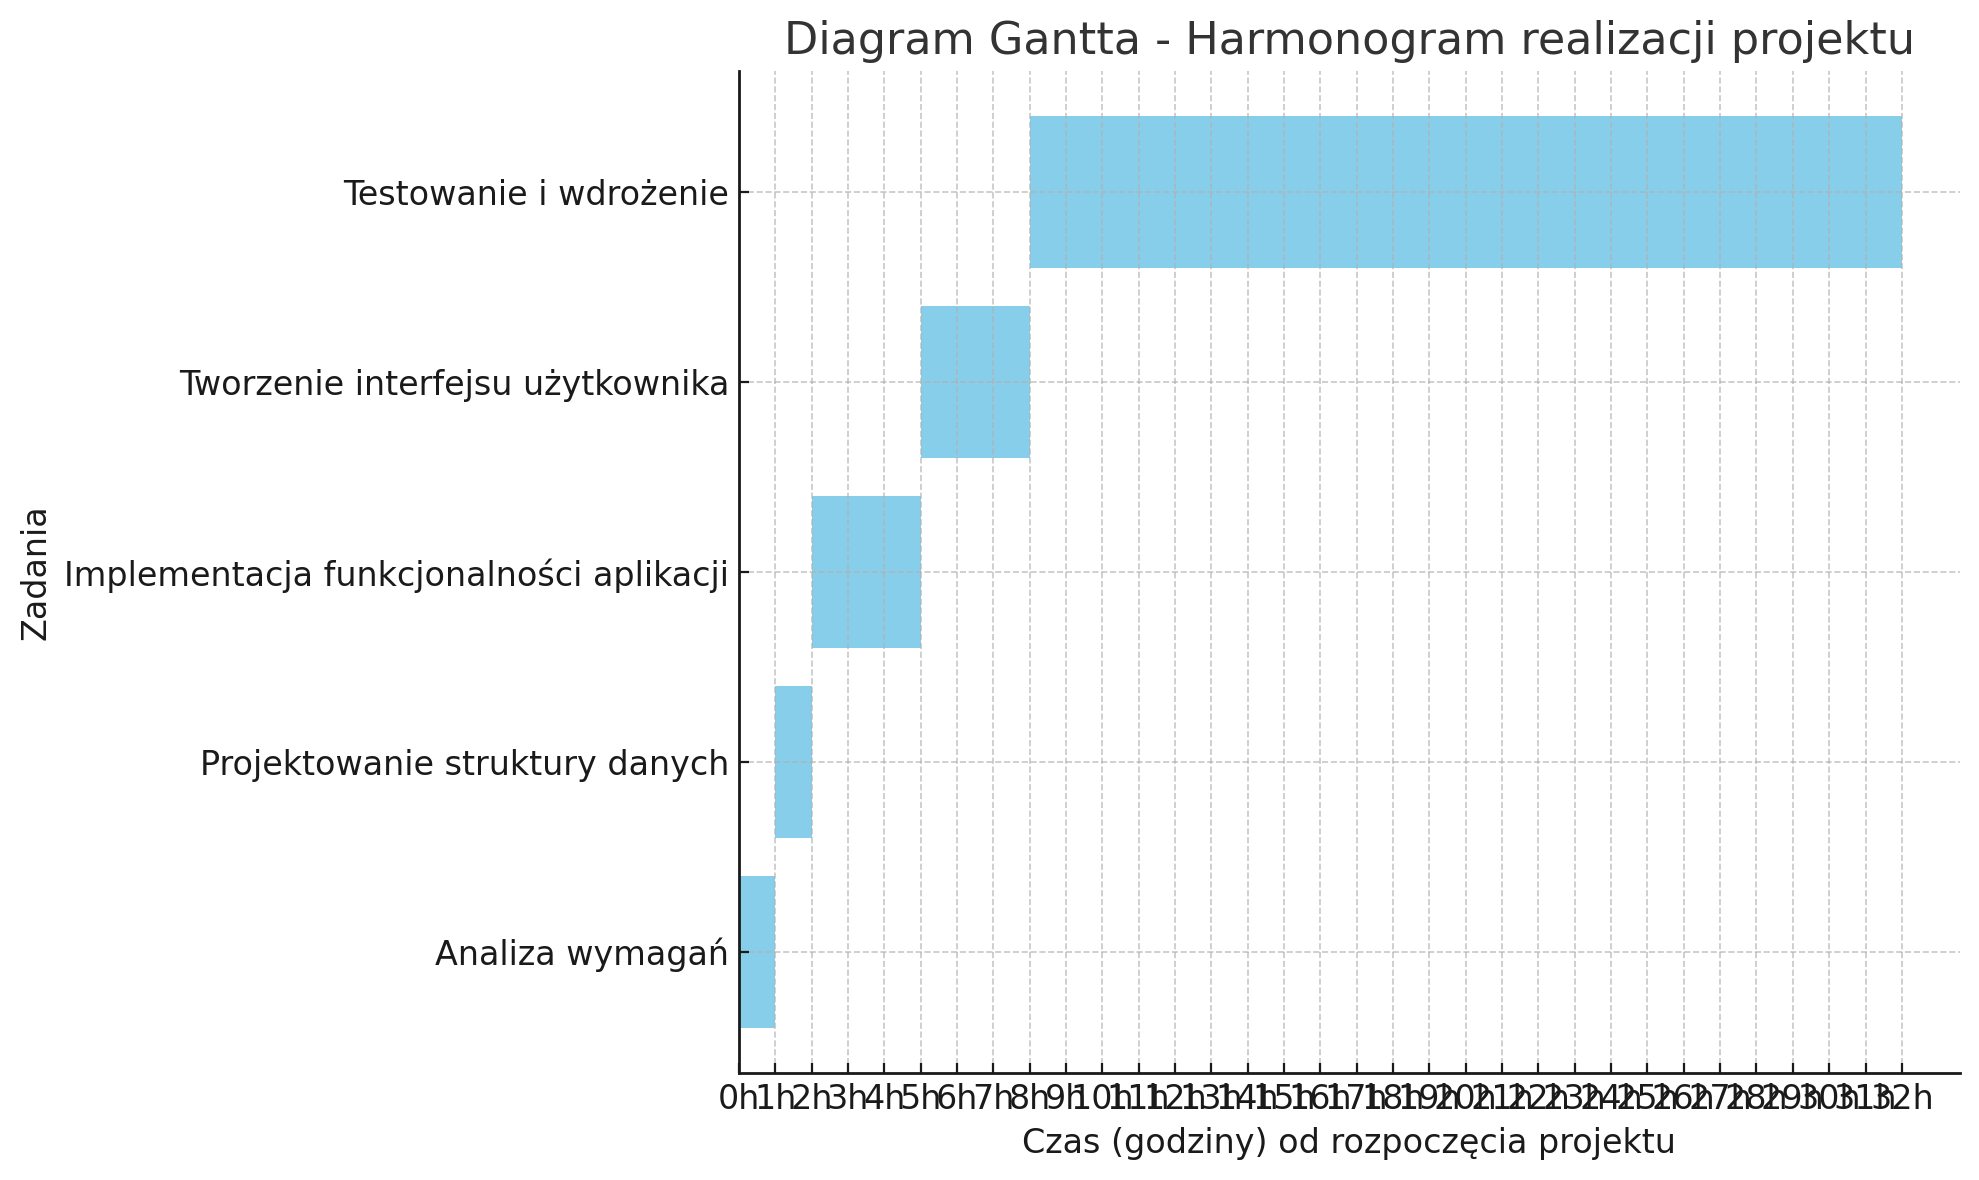
\includegraphics[width=0.8\linewidth]{output (1).png}
    \caption{Rysunek 1. Diagram Ganta}
    \label{fig:enter-label}
\end{figure}

\newpage
\chapter{Prezentacja warstwy użytkowej}
\noindent Aplikacja posiada interfejs użytkownika w formie konsoli, umożliwiający:
\begin{itemize}
    \item Dodawanie i edycję pracowników,
    \item Rejestrowanie godzin pracy i ich zapis do plików tekstowych,
    \item Filtrowanie danych według wybranego zakresu czasu.
\end{itemize}

\noindent Przykładowe zrzuty ekranu aplikacji:
\begin{figure}[h]
    \centering
    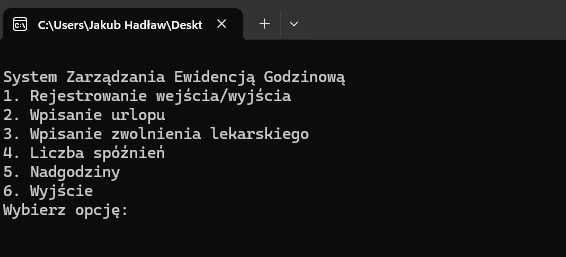
\includegraphics[width=0.8\textwidth]{ss1.png}
    \caption{Główne menu aplikacji}
\end{figure}

\begin{figure}[h]
    \centering
    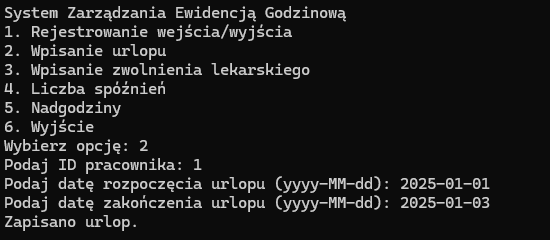
\includegraphics[width=0.8\textwidth]{ss2.png}
    \caption{Ewidencja godzin pracy}
\end{figure}
\begin{figure}[h]
    \centering
    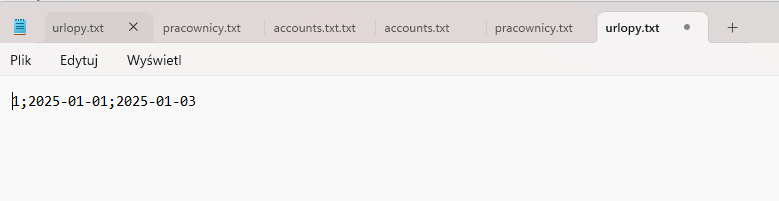
\includegraphics[width=0.8\textwidth]{ss3.png}
    \caption{Zapis w pliku tekstowym}
\end{figure}
\newpage
\chapter{Podsumowanie}
Projekt \textbf{Ewidencja godzinowa pracowników} umożliwia efektywne zarządzanie czasem pracy zatrudnionych osób bez konieczności stosowania baz danych. Dzięki wykorzystaniu plików tekstowych dane są łatwe do przechowywania i edycji.

\noindent Możliwe kierunki dalszego rozwoju obejmują:
\begin{itemize}
    \item Rozszerzenie funkcjonalności o interfejs graficzny,
    \item Możliwość generowania raportów w formacie PDF,
    \item Dodanie automatycznych powiadomień dla pracowników.
\end{itemize}
\newpage


% *************** Zakończenie ***************
% *************** Zakończenie ***************

%***************************************************************************************
% W tym miejscu znajdują się polecenia odpowiedzialne za tworzenie
% spisu ilustracji, spisu treści oraz streszczenia pracy
%***************************************************************************************

%spis rysunków
\addcontentsline{toc}{chapter}{Spis rysunków}
\listoffigures
\newpage


% %streszczenie
% \addcontentsline{toc}{chapter}{Streszczenie}
% \noindent
% {\footnotesize{}\textbf{Wyższa Szkoła Informatyki i Zarządzania z siedzibą w Rzeszowie\\
% Kolegium Informatyki Stosowanej}
% \vspace{30pt}

% \begin{center}
% \textbf{Streszczenie pracy dyplomowej inżynierskiej}\\
% \temat
% \end{center}

% \vspace{30pt}
% \noindent
% \textbf{Autor: \autor
% \\Promotor: \promotor
% \\Słowa kluczowe: tutaj umieść słowa kluczowe}
% \vspace{40pt}
% \\Treść streszczenia, czyli kilka zdań dotyczących treści pracy dyplomowej w języku polskim.
% \vspace{80pt}

% \noindent
% \textbf{The University of Information Technology and Management in Rzeszow\\
% Faculty of Applied Information Technology}
% \vspace{30pt}

% \begin{center}
% \textbf{Thesis Summary\\}
% Tytuł pracy w języku angielskim
% \end{center}

% \vspace{30pt}
% \noindent
% \textbf{Author: \autor
% \\Supervisor: \promotor
% \\Key words: tutaj umieść słowa kluczowe}
% \vspace{40pt}
% \\Treść streszczenia, czyli kilka zdań dotyczących treści pracy dyplomowej w języku angielskim - tłumaczenie tekstu z języka polskiego.
% }

% *************** Koniec pliku back.tex ***************


\end{document}
% *************** Koniec pliku szablon.tex ***************
